%------------------------------------------
\section{Results}
\label{sec:results}

% fs intro
In standard stellar evolution, with no influence from dark matter, stars with \mrange naturally split into two groups with qualitatively different structures, based on the dominant channel through which they burn hydrogen. The dominant channel is determined by the core temperature, with the transition happening at $\Tc \sim 2 \times 10^7 \K$, which corresponds to $\Mstar \sim1.3 \Msun$.

Low mass stars burn hydrogen primarily through the proton-proton (pp) chain for which the burning rate scales with temperature very roughly as $\epspp \propto T^4$. In these stars, the transport of energy away from the core burning region is dominated by photon diffusion. Energy transport in the cores of such stars is said to be radiative.

High mass stars are dominated by the carbon-nitrogen-oxygen (CNO) cycle for which the burning rate scales much more strongly with temperature as $\epsCNO \propto T^{16-20}$. In CNO-dominated stars, radiative energy transport is insufficient to carry away the energy produced by hydrogen burning. Consequently, these high-mass stars have convective cores (not strictly true, let's chat).

\arz{Cite one or more standard references on stellar structure here. I am partially to Kippenhahn, but whatever you like is fine.}.

In \S~\ref{sub:highmass} and \S~\ref{sub:lowmass}, we will consider results for high-mass stars and low-mass stars separately and we will demonstrate that ADM has distinct effects on the evolution of the two groups.
% fe intro

% fs low mass
\subsection{Low-Mass Stars: \mrangelow}
\label{sub:lowmass}

  % 1.0Msun, energy and temperature
  \begin{figure}
    \centering
    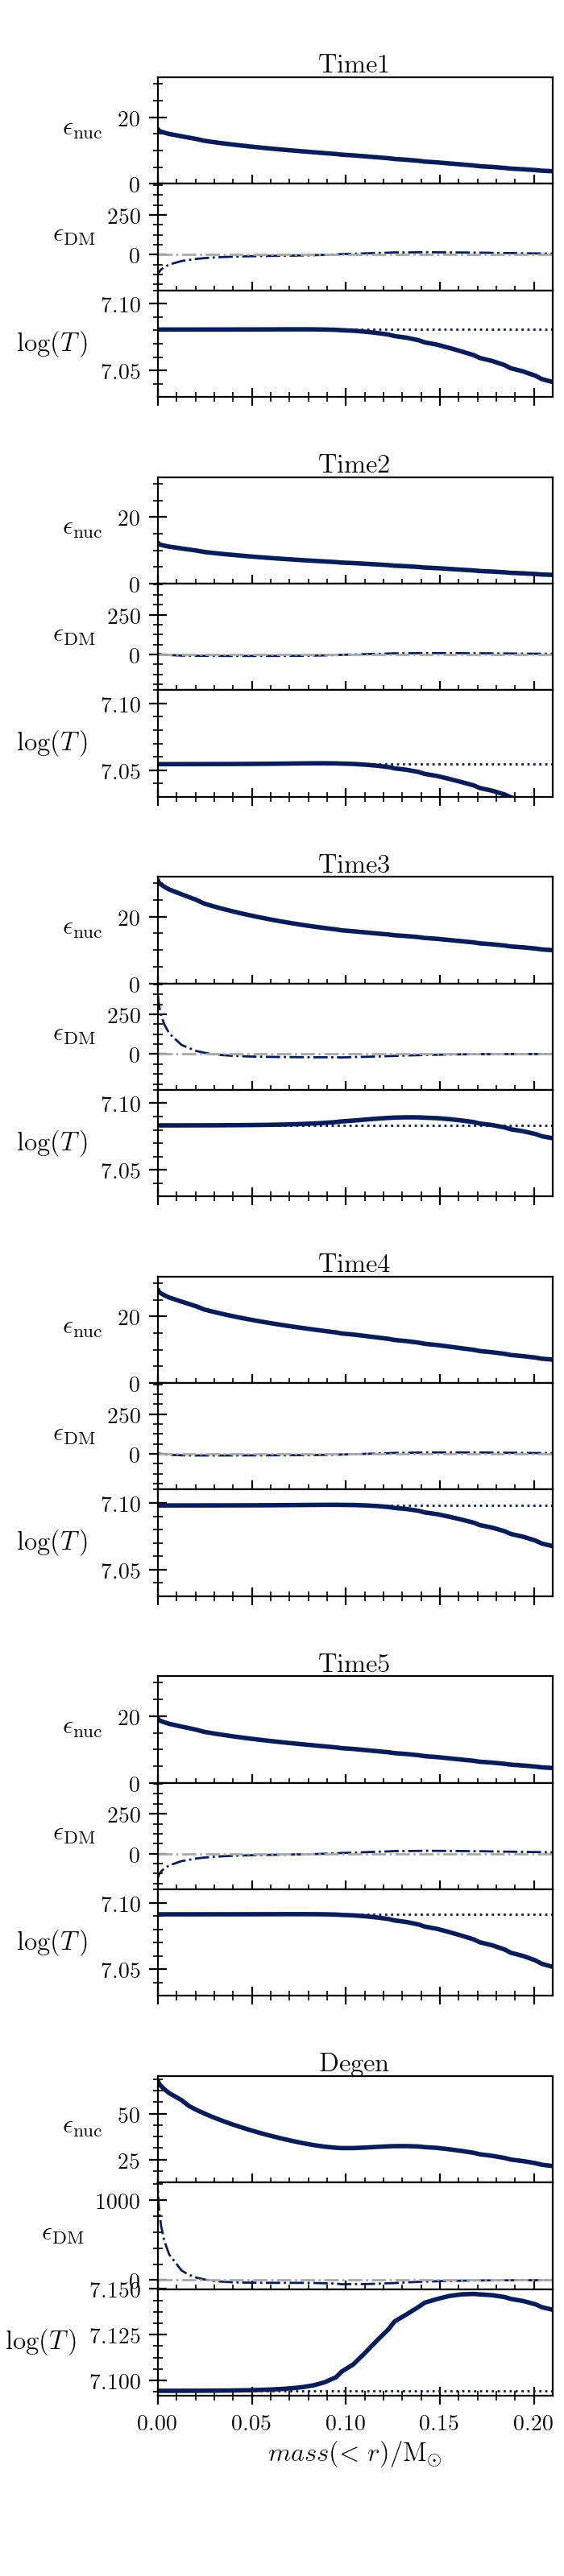
\includegraphics[width=0.47\textwidth]{plots/m1p0c6.png}
    \caption{$1.0 \Msun$ profiles for \nodm (grey) and $\gbpow{6}$ (dark blue) models. In each set of 3 panels, the top 2 are the same as in Figure~\ref{fig:m3p5}. The third panel is the temperature in [K], with the characteristic ADM temperature, $\Tx$, shown as a thin dotted line. ADM energy transport decreases hydrogen burning in the core and pushes the burning into a shell more quickly than the reference models. The reduced central burning causes the $\gbpow{3}$ model to live slightly longer than the \nodm model.
    }
    \label{fig:m1p0_a}
  \end{figure}


Standard model stars in this mass range have relatively low central temperatures and so are powered primarily by the pp chain, which is much less sensitive to the temperature than burning via the CNO cycle. This means the burning does not peak as strongly at the center and radiative transport is sufficient to carry the energy flux, so the core is radiative, not convective. Without convective mixing, hydrogen depletes first at the very center and the burning shifts outward gradually.

As stars with $\gb$ as low as $10^2$ (check this number) enter the MS, ADM is already transporting a significant amount of energy away from the center ($\epsx \approx \epspp$ near $r=0$) and depositing it in a shell at $m(<r) \approx 0.1 \Msun$. This causes the temperature, and therefore the burning rate, to be lower at the center and higher in a shell relative to standard models.

% fe low mass

% fs high mass
\subsection{High-Mass Stars: \mrangehigh}
\label{sub:highmass}

  % 3.5Msun, energy and convection
  \begin{figure}
    \centering
    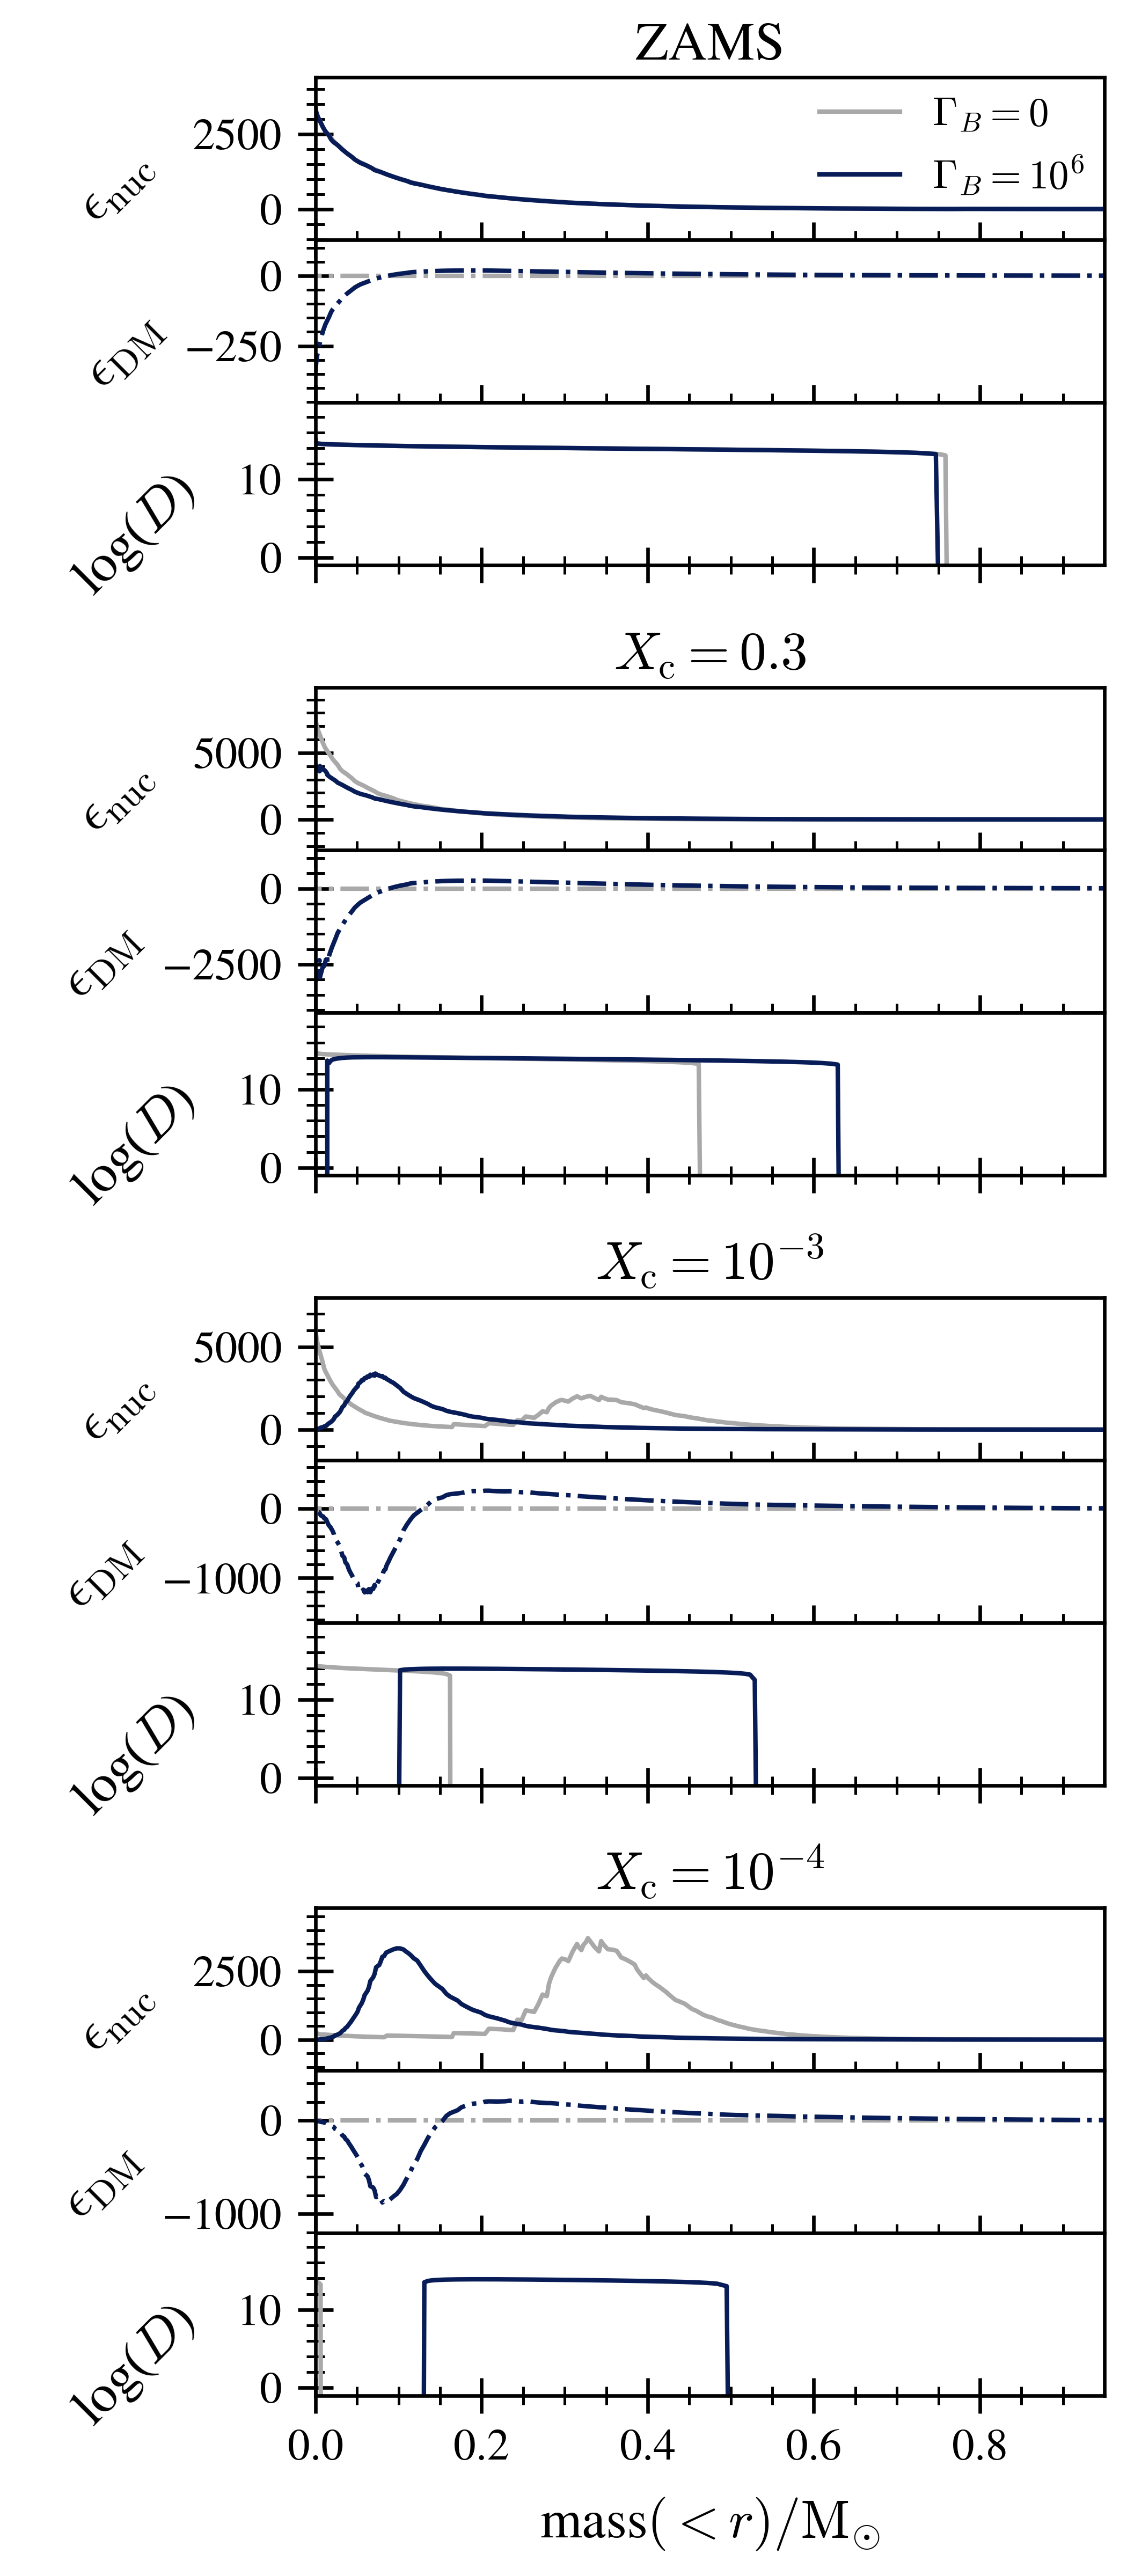
\includegraphics[width=0.47\textwidth]{plots/m3p5.png}
    \caption{$3.5 \Msun$ profiles for \nodm (grey) and $\gbpow{6}$ (dark blue) models. Each set of 3 panels shows stellar profiles of the stars at different evolutionary phases indicated by the fraction of hydrogen in the center, $X_c$, which decreases as the star evolves. The profiles in each panel are: 1) $\epsnuc$, the nuclear burning rate in [erg/g/s], 2) $\epsdm$, the rate at which DM transports energy (negative values indicate that energy is being removed), also in [erg/g/s], 3) D, the diffusion coefficient for convective + overshoot mixing in [cm$^2$/s]. In the \nodm model the convective core retreats toward the center over time, and the burning rate peaks at the center until the end of the main sequence when the central burning rate drops dramatically and a shell of strong burning appears. In the $\gbpow{6}$ model, convection at the very center shuts off early in the MS and a convective shell retreats away from the center over time. The peak burning rate shifts gradually outward, following the inner edge of the convective shell.
    }
    \label{fig:m3p5}
  \end{figure}

In standard models, MS stars with $\Mstar \gtrsim 1.3 \Msun$ are powered primarily by the CNO cycle.
This has several important consequences:
(1) the burning rate is much higher than in pp-dominated stars;
(2) the burning rate is extremely sensitive to core temperature;
and (3) stellar cores must be convective in order to carry away the energy produced by core hydrogen burning.
Once hydrogen throughout the convective zone is depleted, the burning rate rapidly decreases, and the star loses more energy at its surface than is being generated by burning. Gravity temporarily dominates over the pressure support from burning and the star contracts until the internal temperature increase is sufficient to ignite hydrogen in a shell outside the depleted core. See Figure~\ref{fig:m3p5}.

If a star captures enough ADM, the combination of dark matter + radiative energy transport becomes sufficient to carry the flux from nuclear burning. Convection disappears from the center first (where ADM energy transport is most efficient) and retreats away from the core, into a narrowing shell. Without convective mixing, the central hydrogen supply depletes (I don't think this is the right reason) and the burning also shifts into a shell, following the lower boundary of the convective zone. This can be seen in the time progression (down the page) of the $\gbpow{6}$ (dark blue) model in Figure~\ref{fig:m3p5}. The shift to shell burning is more similar to the behavior of standard low mass models.

% fe high mass

% fs MS lifetimes
% mstau plot
\begin{figure*}
  \centering
  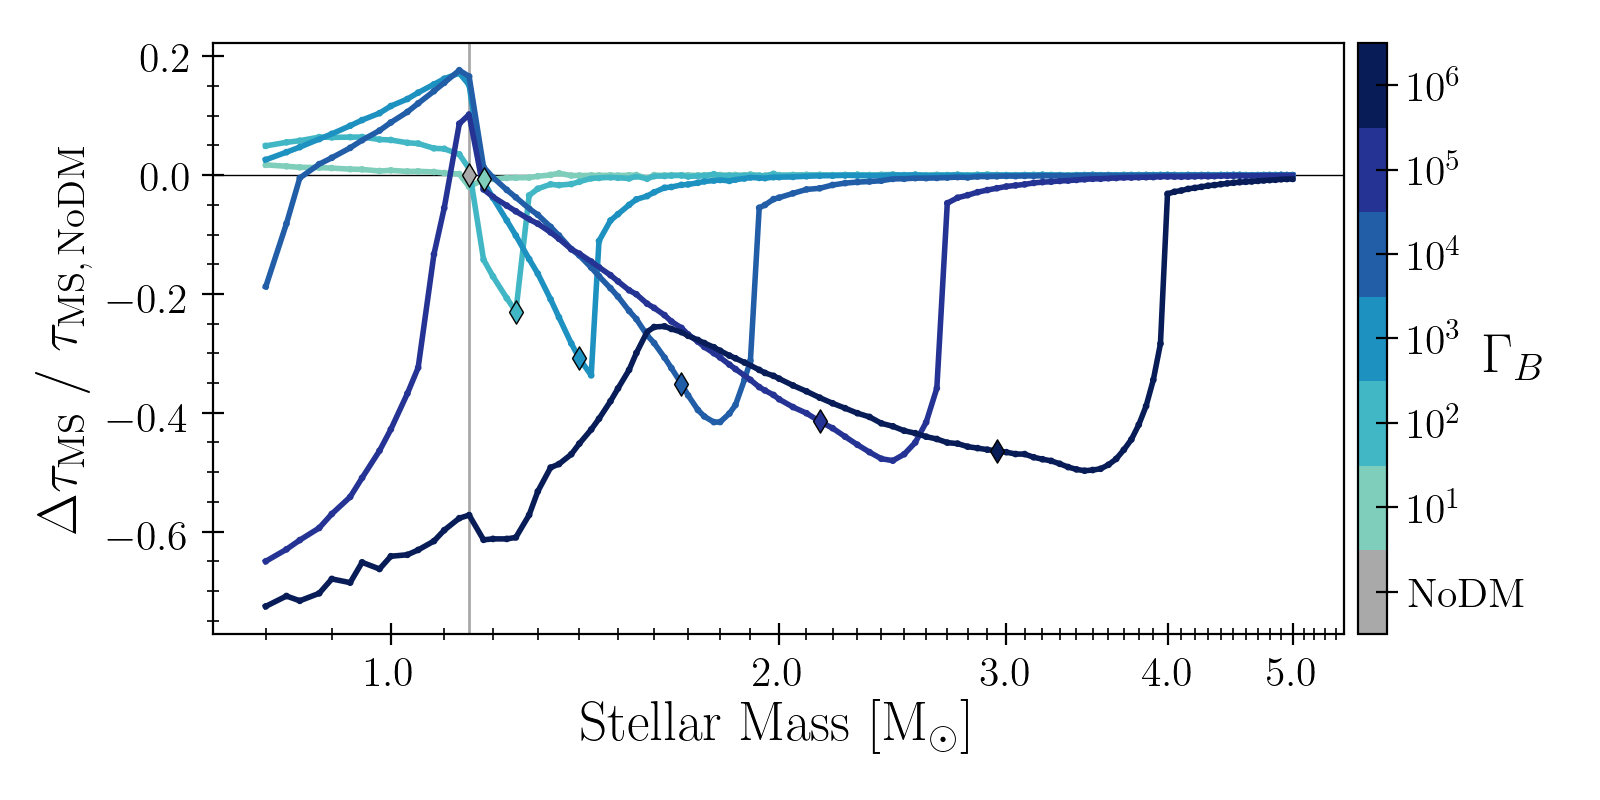
\includegraphics[width=\textwidth]{plots/mstau.png}
  \caption{The presence of ADM tends to shorten MS lifetimes relative to models with no dark matter.
  Diamonds mark the transition from radiative to convective cores (left to right). For the purposes of this figure this is defined as the lowest \Mstar for which the average (over the MS) mass of the convective core is greater than 0.01 Mstar. This transition is also marked by a vertical line for the \nodm model since this is what splits the low and high mass groups. Stars to the right of this line have decreased lifetimes due to a reduction in the size of the convective core, which reduces the amount of hydrogen available for burning. The effect abruptly disappears as stellar lifetimes become shorter than the time required to build up a sufficient amount of ADM. Stars to the left of the vertical line show mixed behavior. Those with lower $\gb$ have increased lifetimes due to decreased burning rates. Those with high $\gb$ show little change.
  }
  \label{fig:mstau}
\end{figure*}

In Fig.~\ref{fig:mstau} we show the effects of ADM on main sequence (MS) lifetimes relative to a standard \nodm star of the same mass. We have defined the MS to end when the fractional abundance of hydrogen in the center, $X_c$, falls below $10^{-3}$ (check the number, MIST defines TAMS = 10^-12). $X_c$ declines rapidly at the end of the MS, so our results are not strongly affected by the exact choice.

Lifetimes of low mass stars, which have radiative (not convective) cores even in \nodm models, are not greatly affected by ADM. Models with intermediate \gammaB values have their lifetimes extended by up to $~20\%$ because the DM energy transport reduces the temperature in the center, which in turn reduces the burning rate. Models that capture large amounts of ADM (high \gammaB values) have very little change in their MS lifetimes. (why? Perhaps the burning rate in the shell is high enough, and the settling happens fast enough that helium ash accumulates in the core at the same rate as in no DM models?)

ADM tends to shorten the lifetimes of high mass stars ($\Mstar \gtrsim 1.3 \Msun$), an effect that increases with \gammaB. In \nodm models, the central convection zone extends beyond the burning region, giving the star a source of fresh nuclear fuel as hydrogen from outside of the core is mixed into the center. Since ADM shuts off convection in the center, the star no longer gets this influx of unburnt hydrogen, therefore it has less fuel to burn and so it leaves the MS faster than the \nodm models. Note that the appearance of the convective core shifts to higher masses with increasing \gammaB (diamonds in Fig.~\ref{fig:mstau}) due to larger amounts of ADM which can carry larger energy fluxes. The effects disappear abruptly as $\Mstar$ approaches $5 \Msun$ because stellar lifetimes (which scale as $\Mstar^{-2.5}$ (check exact number)) quickly become too short for a sufficient amount of ADM to build up in the star (recall that the ADM capture rate scales linearly with $\Mstar$).

% fe MS lifetimes

% fs isochrones
% isochrones plots
\begin{figure*}
  \centering
  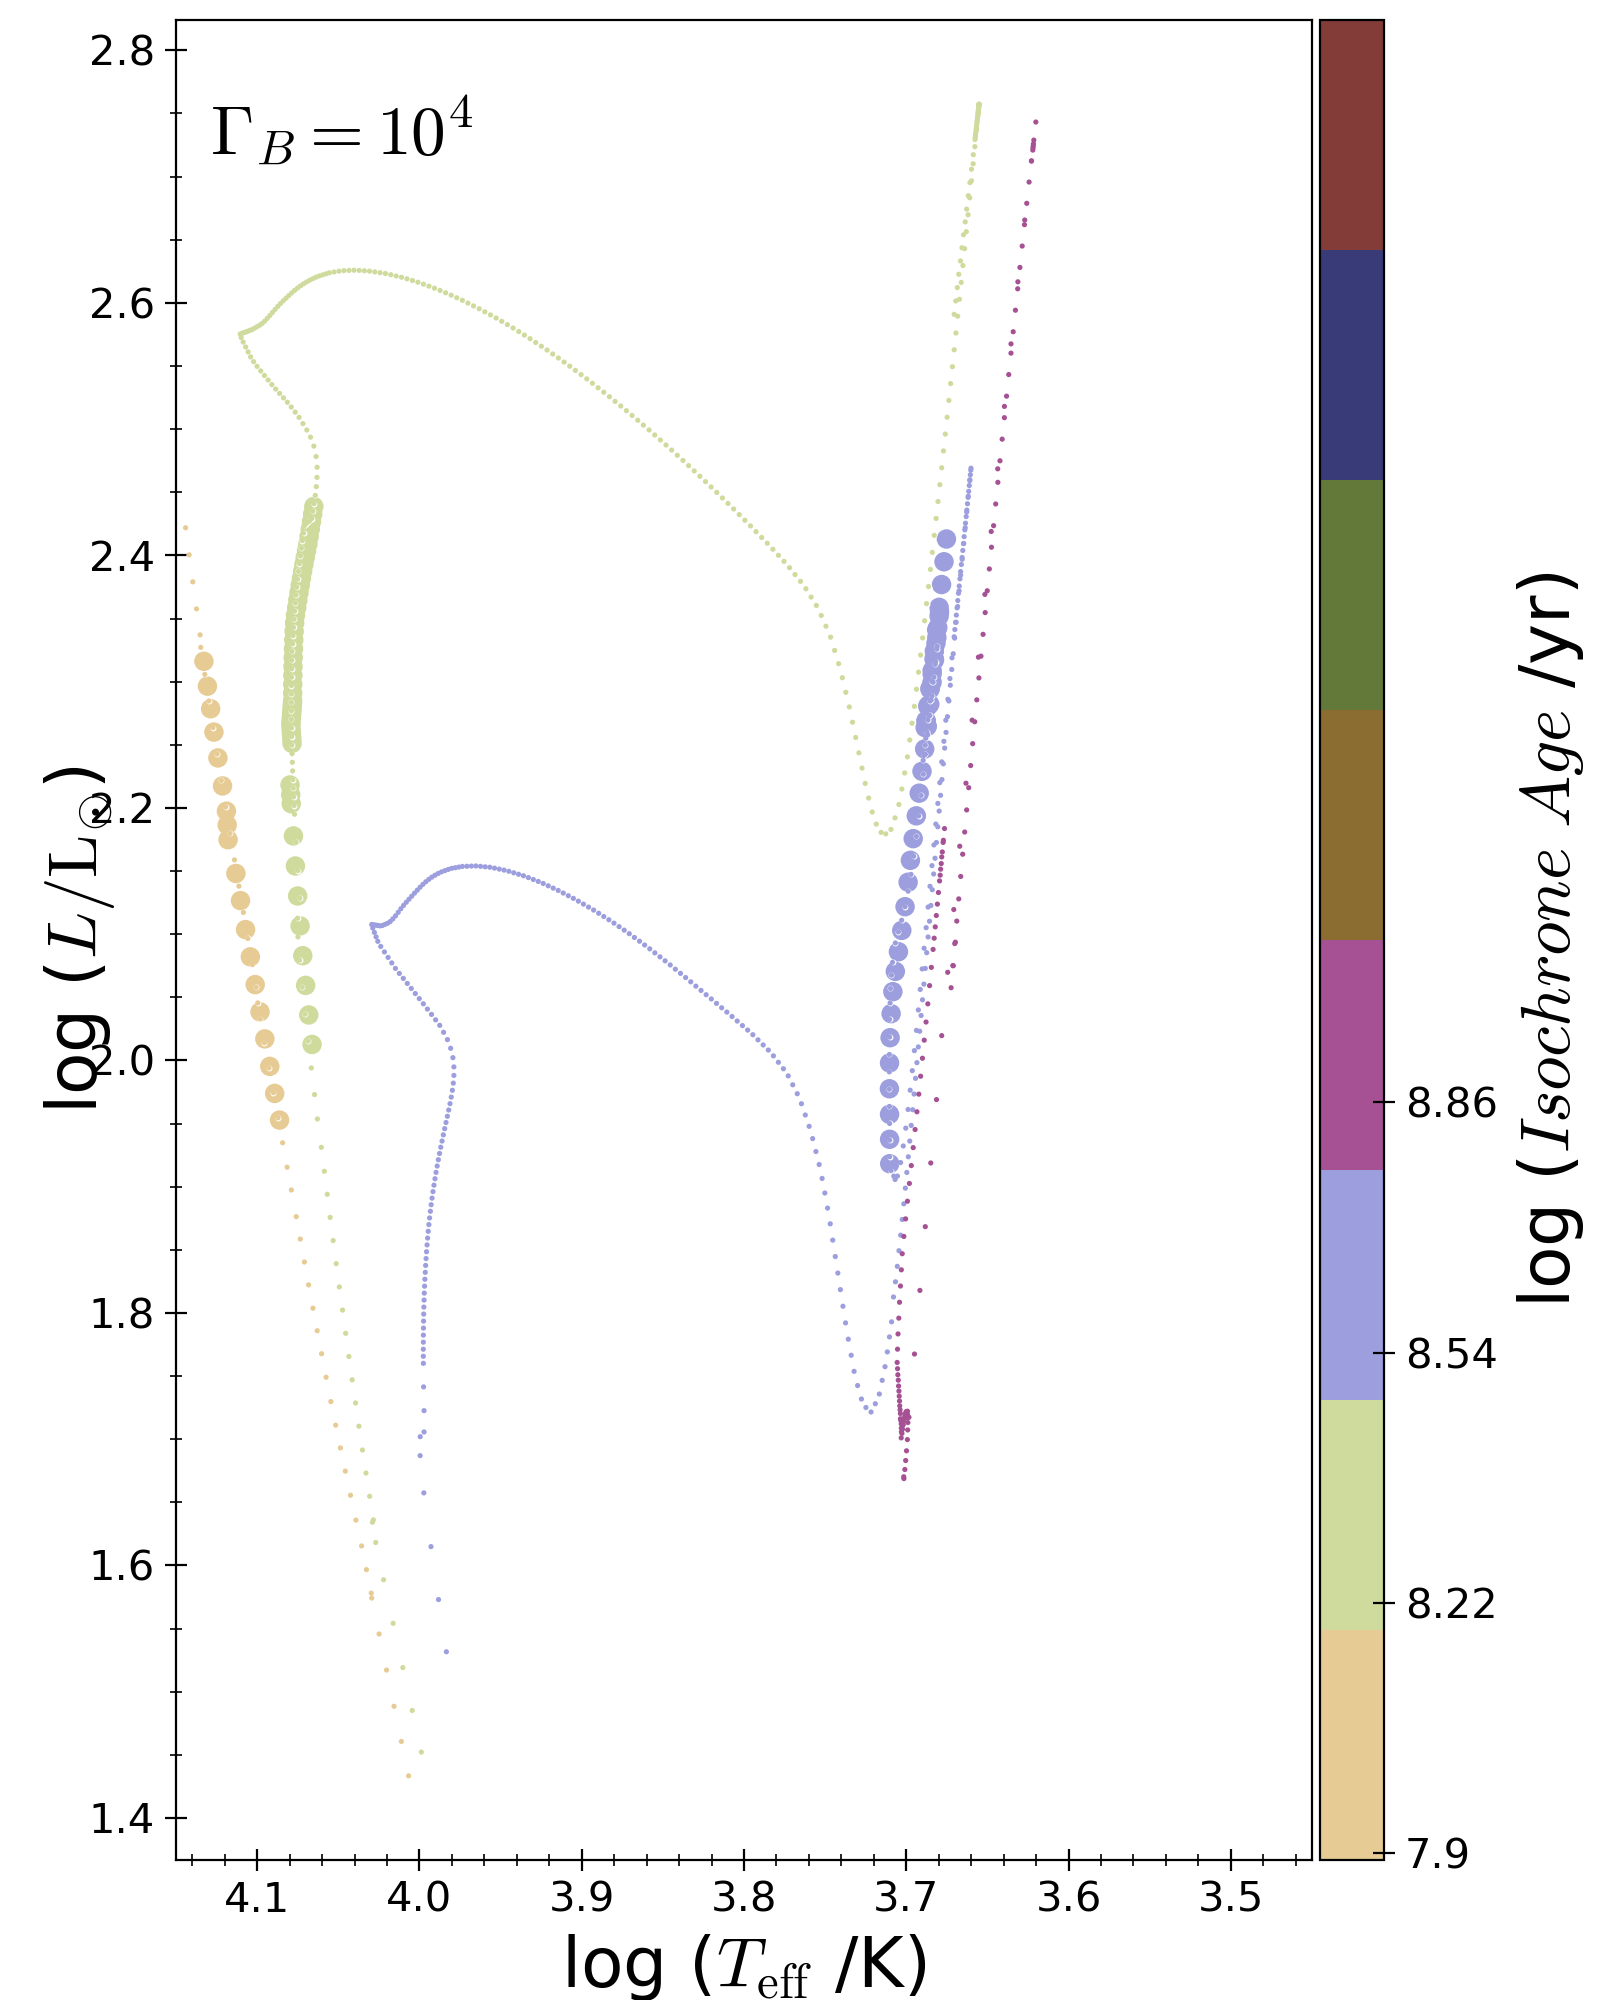
\includegraphics[width=\textwidth]{plots/isos_cb4.png}
  \caption{$\gbpow{4}$ isochrones with \nodm models overplotted as thin lines. Triangles mark $3.5 \Msun$, circles mark $1.0 \Msun$. The positions of the markers here are very similar to the \nodm case (not shown). Gaps in the data are due to the difficulty interpolating in regions where the stellar mass - age relation of a given EEP (equivalent evolutionary phase) is non-monotonic. This is a known problem that Dotter discusses in his paper.
  }
  \label{fig:isos_cb4}
\end{figure*}

\begin{figure*}
  \centering
  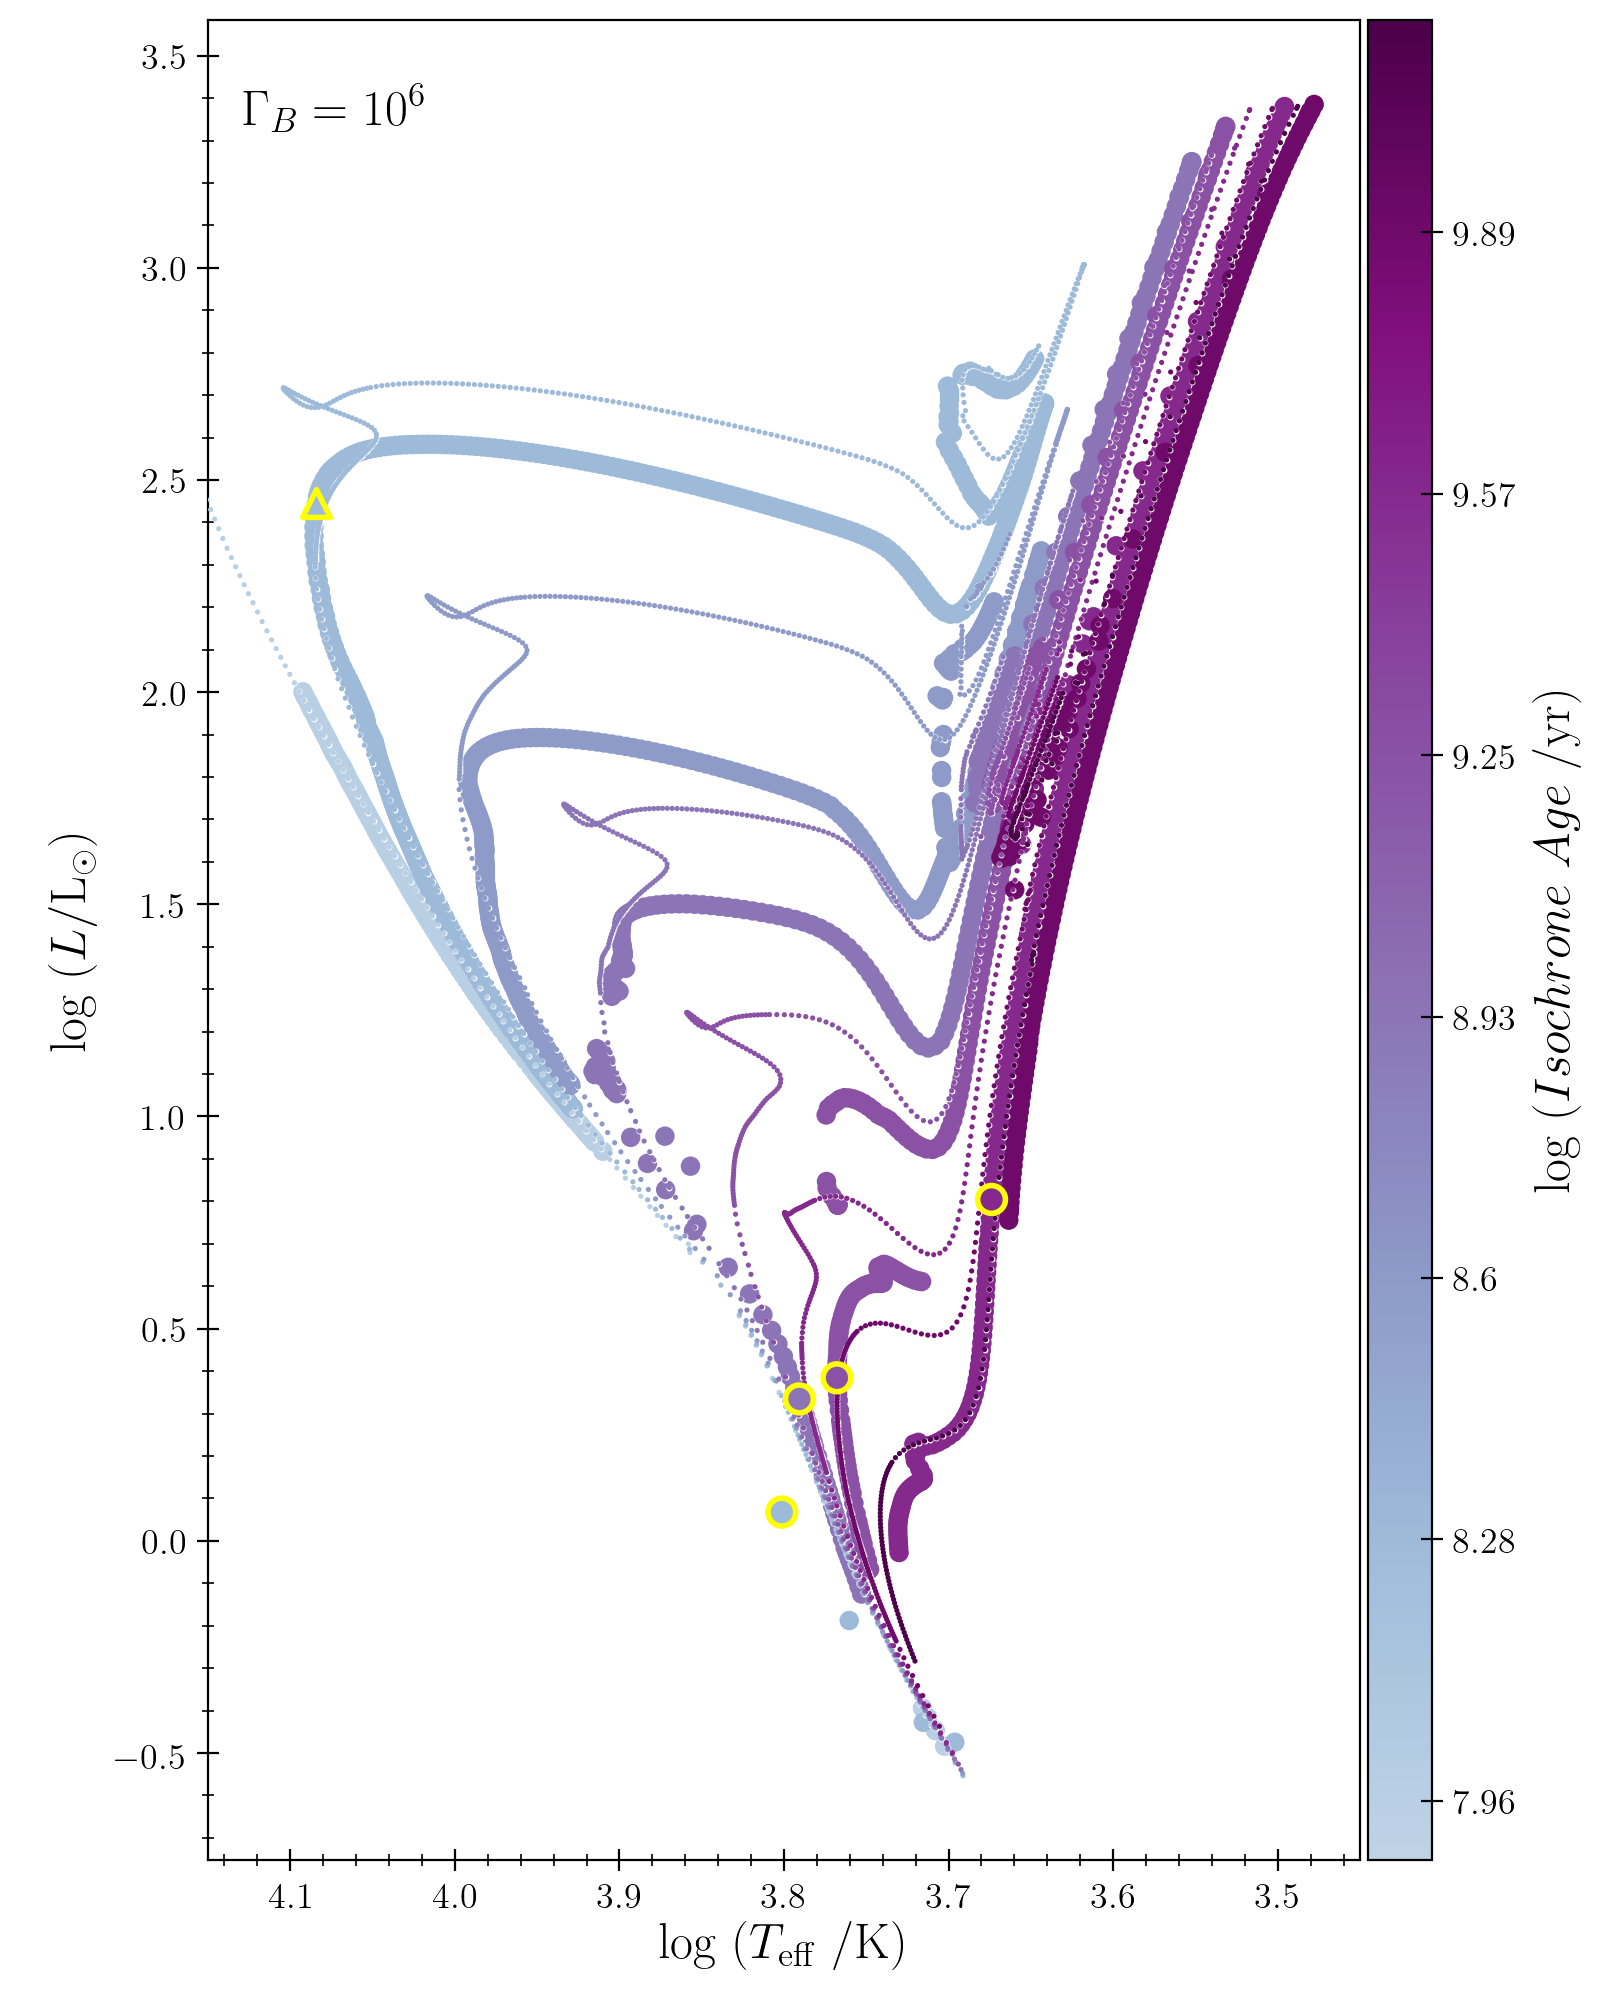
\includegraphics[width=\textwidth]{plots/isos_cb6.png}
  \caption{Same as Fig.~\ref{fig:isos_cb4} but for $\gbpow{6}$.
  }
  \label{fig:isos_cb6}
\end{figure*}


% hottest MS Teff plots
\begin{figure*}
    \centering
    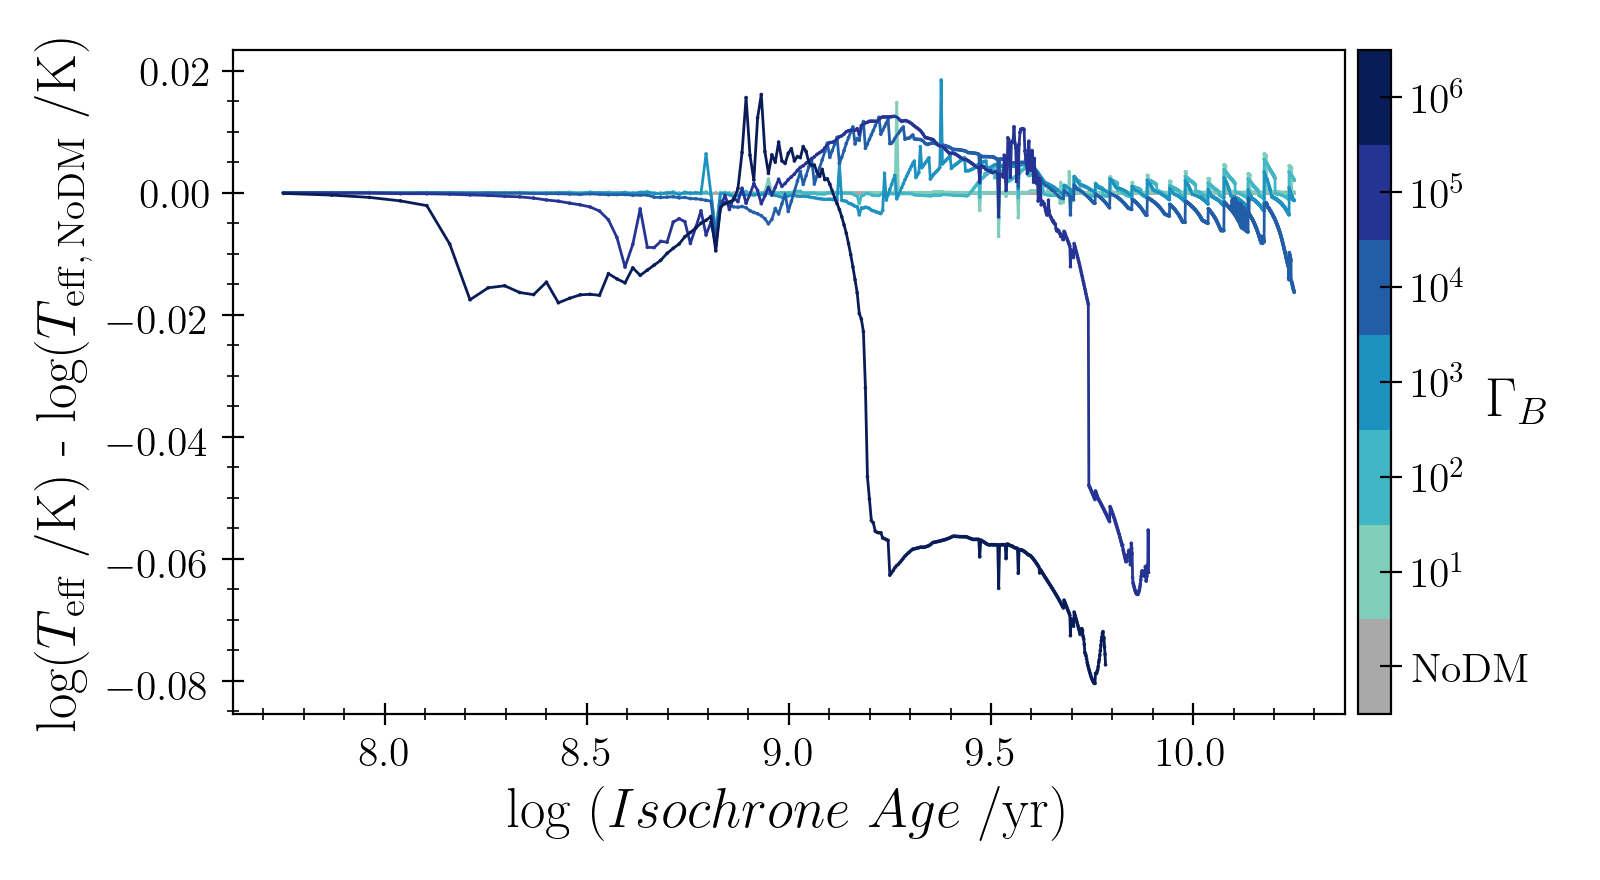
\includegraphics[width=\textwidth]{plots/hotTeff_resid.png}
    \caption{
    Main sequence turnoff temperature (temperature of the hottest star that is still on the main sequence). Residuals are with respect to (...?)
    }
    \label{fig:hotTeff}

\end{figure*}


Define/describe isochrones here?

We find that, for stars significantly affected by ADM energy transport, the general effect is to shorten MS lifetimes (see Figure \ref{fig:mstau}) so that, for a stellar populations of a given age, the MS turn-off happens at a lower mass and the stars evolve through the sub-giant branch at a lower luminosity (see Figure \ref{fig:isos}). This causes isochrones of clusters in high $\gb$ environments to appear older than their standard model counterparts. This becomes noticeable in the highest $\gb$ environments around 0.2 Gyr as stars with $\rm{M} \approx 4 \Msun$ begin to leave the MS. Prior to this the stars have not had enough time to capture a sufficient number of DM particles for ADM-driven energy transport to be a significant contribution to the overall energy transfer within the star.  This behavior (burning shifting into a shell) is very similar to high-mass stars that collect large amounts of ADM, which contributes to isochrones appearing older as $\gb$ gets large.

Hi mass: The result is that these stars leave the MS earlier and at a lower luminosity, and they skip the convective hook altogether (Figure \ref{fig:tracks}). This makes the isochrones appear older than their `\nodm' counterparts (Figure \ref{fig:isos_cb}).


% fe isochrones
